\section{作品欣賞}
\begin{center}
\begin{figboxs}
\centering
\includegraphics[height = \textheight]{快門.pdf}
\end{figboxs}
\end{center}
\newpage
%%%%%
\begin{center}
\begin{figboxs}
\centering
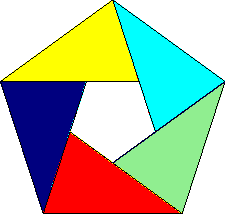
\includegraphics[height = \textheight]{五芒星.pdf}
\end{figboxs}
\end{center}
\newpage
%%%%%
\begin{center}
\begin{figboxs}
\centering
\includegraphics[height = \textheight]{音韻季.pdf}
\end{figboxs}
\end{center}
\newpage
%%%%%
\begin{center}
\begin{figboxs}
\centering
\includegraphics[height = \textheight]{煙火.pdf}
\end{figboxs}
\end{center}
\newpage
%%%%%
\begin{center}
\begin{figboxs}
\centering
\includegraphics[height = \textheight]{曼陀羅.pdf}
\end{figboxs}
\end{center}
\newpage
%%%%%
\begin{center}
\begin{figboxs}
\centering
\includegraphics[height = \textheight]{星河.pdf}
\end{figboxs}
\end{center}
\newpage
%%%%%
\begin{center}
\begin{figboxs}
\centering
\includegraphics[height = \textheight]{五瓣花.pdf}
\end{figboxs}
\end{center}
\newpage
%%%%%
\begin{center}
\begin{figboxs}
\centering
\includegraphics[height = \textheight]{異想天開.pdf}
\end{figboxs}
\end{center}
\newpage
%%%%%
\begin{center}
\begin{figboxs}
\centering
\includegraphics[height = \textheight]{楓葉.pdf}
\end{figboxs}
\end{center}
\newpage
%%%%%
\myvcenter{\huge}{以上皆為程式語言繪製}
\newpage
%%%%%
\myvcenter{\huge}{為什麼要用程式語言繪圖?}
\newpage
%%%%%
\section{你的右上角不是我的右上角}
\begin{tcolorbox}[width = \textwidth]
\centering
你的右上角不是我的右上角
\end{tcolorbox}
\vskip0.5cm
\begin{center}
\begin{tikzpicture}
\draw (2,2) rectangle (-2,-2);
\draw[<-] (2.5,0)--(-2.5,0);
\draw[<-] (0,2.5)--(0,-2.5);
\end{tikzpicture}
\end{center}
%%%%%
\begin{luacode}
local arr = {
	"(2,2)",
	"(1.8,1.8)",
	"(1.9,1.9)",
	"(1.7,1.9)",
	"(1.9,1.7)",
	"(1.6,1.9)",
	"(2,1.9)", 
	"(1.9,2)", 
	"(1.9,1.8)", 
	"(2.07,2.07)"
 }
for i = 1,10 do
tex.sprint("\\newpage")
tex.sprint("\\begin{tcolorbox}[width = \\textwidth]")
tex.sprint("\\centering")
tex.sprint("你的右上角不是我的右上角")
tex.sprint("\\end{tcolorbox}")
tex.sprint("\\vskip0.5cm")
tex.sprint("\\begin{center}")
tex.sprint("\\begin{tikzpicture}")
tex.sprint("\\draw (2,2) rectangle (-2,-2);")
tex.sprint("\\draw[<-] (2.5,0)--(-2.5,0);")
tex.sprint("\\draw[<-] (0,2.5)--(0,-2.5);")
for x = 1,i do
tex.sprint("\\draw ".. arr[x] .." circle (0.1);")
end
tex.sprint("\\end{tikzpicture}")
tex.sprint("\\end{center}")
end
\end{luacode}
\newpage
%%%%%
\begin{tcolorbox}[width = \textwidth]
\centering
在 $(2,2)$ 上的一點
\end{tcolorbox}
\vskip0.5cm
\begin{center}
\begin{tikzpicture}
\draw (2,2) rectangle (-2,-2);
\draw[<-] (2.5,0)--(-2.5,0);
\draw[<-] (0,2.5)--(0,-2.5);
\draw (2,2) circle (0.1);
\end{tikzpicture}
\end{center}
\newpage
%%%%%
\begin{tcolorbox}[width = \textwidth]
\centering
在 $[\sqrt{8}:45^\circ]$ 上的一點
\end{tcolorbox}
\vskip0.5cm
\begin{center}
\begin{tikzpicture}
\draw (2,2) rectangle (-2,-2);
\draw[<-] (2.5,0)--(-2.5,0);
\draw[<-] (0,2.5)--(0,-2.5);
\draw (45:{sqrt(8)}) circle (0.1);
\end{tikzpicture}
\end{center}
\newpage
%%%%%
\begin{tcolorbox}[width = \textwidth]
\centering
在 $[\sqrt{8}:\left(\frac{\pi}{4}\right)]$ 上的一點
\end{tcolorbox}
\vskip0.5cm
\begin{center}
\begin{tikzpicture}
\draw (2,2) rectangle (-2,-2);
\draw[<-] (2.5,0)--(-2.5,0);
\draw[<-] (0,2.5)--(0,-2.5);
\draw (45:{sqrt(8)}) circle (0.1);
\end{tikzpicture}
\end{center}
\newpage
%%%%%
\begin{tcolorbox}[width = \textwidth]
\centering
在 $(2\sqrt{2}\times\sin(45^\circ),2\sqrt{2}\times\cos(45^\circ))$ 上的一點
\end{tcolorbox}
\vskip0.5cm
\begin{center}
\begin{tikzpicture}
\draw (2,2) rectangle (-2,-2);
\draw[<-] (2.5,0)--(-2.5,0);
\draw[<-] (0,2.5)--(0,-2.5);
\draw (2,2) circle (0.1);
\end{tikzpicture}
\end{center}
\newpage
%%%%%
\centerbox{數學描述是不會變動的}
\newpage
%%%%%
\section{幾何之美}
\begin{tcolorbox}
幾何之美
\end{tcolorbox}
\begin{figbox}
\centering
\includegraphics[height = \textheight -72pt]{快門.pdf}
\end{figbox}
\newpage
%%%%%
\begin{tcolorbox}
幾何之美
\end{tcolorbox}
\begin{figbox}
\centering
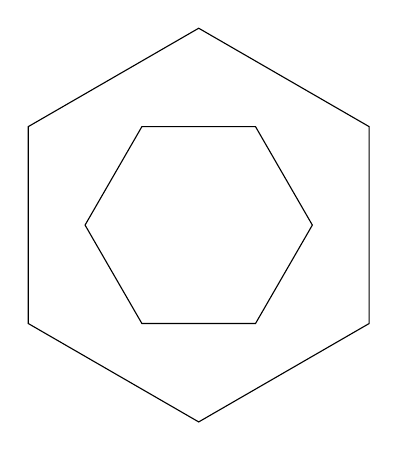
\begin{tikzpicture}
\draw (30:2.5)--(90:2.5)--(150:2.5)--(210:2.5)--(270:2.5)--(330:2.5)--cycle;
\draw (0:{(2.5/sqrt(3))})--(60:{(2.5/sqrt(3))})--(120:{(2.5/sqrt(3))})--(180:{(2.5/sqrt(3))})--(240:{(2.5/sqrt(3))})--(300:{(2.5/sqrt(3))})--cycle;
\end{tikzpicture}
\end{figbox}
\newpage
%%%%%
\begin{tcolorbox}
計算過程
\end{tcolorbox}
\begin{figbox}
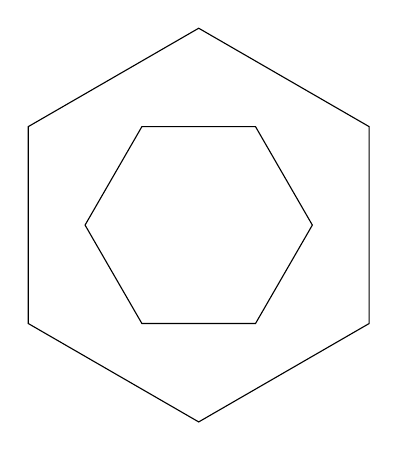
\begin{tikzpicture}
\draw (30:2.5)--(90:2.5)--(150:2.5)--(210:2.5)--(270:2.5)--(330:2.5)--cycle;
\draw (0:{(2.5/sqrt(3))})--(60:{(2.5/sqrt(3))})--(120:{(2.5/sqrt(3))})--(180:{(2.5/sqrt(3))})--(240:{(2.5/sqrt(3))})--(300:{(2.5/sqrt(3))})--cycle;
\end{tikzpicture}
\end{figbox}
\newpage
%%%%%
\begin{tcolorbox}
計算過程
\end{tcolorbox}
\begin{figbox}
\begin{multicols}{2}
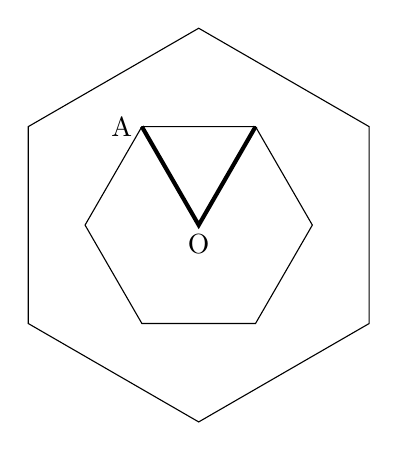
\begin{tikzpicture}
\draw (30:2.5)--(90:2.5)--(150:2.5)--(210:2.5)--(270:2.5)--(330:2.5)--cycle;
\draw (0:{(2.5/sqrt(3))})--(60:{(2.5/sqrt(3))})--(120:{(2.5/sqrt(3))})--(180:{(2.5/sqrt(3))})--(240:{(2.5/sqrt(3))})--(300:{(2.5/sqrt(3))})--cycle;
\draw[line width = 1.5pt] (60:{(2.5/sqrt(3))})--(0,0)--(120:{(2.5/sqrt(3))});
\node[below] at(0,0) {O};
\node[left] at(120:{(2.5/sqrt(3))}) {A};
\end{tikzpicture}
\columnbreak

$\overline{OA} = 2$
\end{multicols}
\end{figbox}
\newpage
%%%%%
\begin{tcolorbox}
計算過程
\end{tcolorbox}
\begin{figbox}
\begin{multicols}{2}
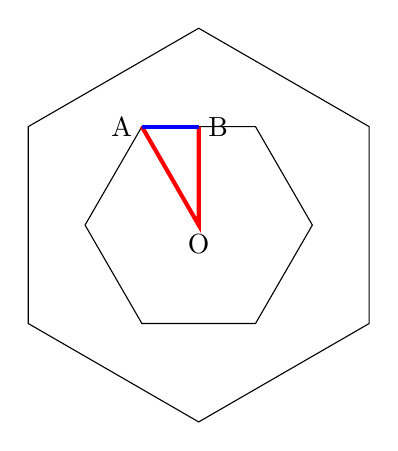
\begin{tikzpicture}
\draw (30:2.5)--(90:2.5)--(150:2.5)--(210:2.5)--(270:2.5)--(330:2.5)--cycle;
\draw (0:{(2.5/sqrt(3))})--(60:{(2.5/sqrt(3))})--(120:{(2.5/sqrt(3))})--(180:{(2.5/sqrt(3))})--(240:{(2.5/sqrt(3))})--(300:{(2.5/sqrt(3))})--cycle;
\draw[line width = 1.5pt, red] (120:{(2.5/sqrt(3))})--(0,0)--(90:{(2.5/sqrt(3))*sqrt(3)/2});
\draw[line width = 1.5pt, blue] (120:{(2.5/sqrt(3))})--(90:{(2.5/sqrt(3))*sqrt(3)/2});
\node[below] at(0,0) {O};
\node[left] at(120:{(2.5/sqrt(3))}) {A};
\node[right] at(90:{(2.5/sqrt(3))*sqrt(3)/2}) {B};
\end{tikzpicture}
\columnbreak


$\overline{OA} = 2$
\\
$\overline{AB} = 1$
\\
$\overline{OB} = \sqrt{3}$
\end{multicols}
\end{figbox}
\newpage
%%%%%

\begin{tcolorbox}
計算過程
\end{tcolorbox}
\begin{figbox}
\begin{multicols}{2}
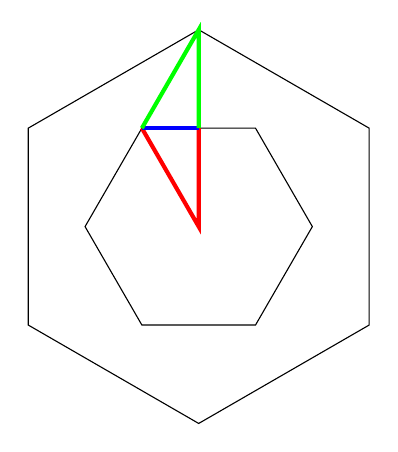
\begin{tikzpicture}
\draw (30:2.5)--(90:2.5)--(150:2.5)--(210:2.5)--(270:2.5)--(330:2.5)--cycle;
\draw (0:{(2.5/sqrt(3))})--(60:{(2.5/sqrt(3))})--(120:{(2.5/sqrt(3))})--(180:{(2.5/sqrt(3))})--(240:{(2.5/sqrt(3))})--(300:{(2.5/sqrt(3))})--cycle;
\draw[line width = 1.5pt, red] (120:{(2.5/sqrt(3))})--(0,0)--(90:{(2.5/sqrt(3))*sqrt(3)/2});
\draw[line width = 1.5pt, blue] (120:{(2.5/sqrt(3))})--(90:{(2.5/sqrt(3))*sqrt(3)/2});
\draw[line width = 1.5pt, green] (120:{(2.5/sqrt(3))})--(90:2.5)--(90:{(2.5/sqrt(3)*sqrt(3)/2)});
\end{tikzpicture}
\columnbreak


$\overline{OA} = 2$
\\
$\overline{AB} = 1$
\\
$\overline{OB} = \sqrt{3}$
\end{multicols}
\end{figbox}
\newpage
%%%%%
\begin{tcolorbox}
計算過程
\end{tcolorbox}
\begin{figbox}
\begin{multicols}{2}
\begin{tikzpicture}
\draw[draw = none] (30:2.5)--(90:2.5)--(150:2.5)--(210:2.5)--(270:2.5)--(330:2.5)--cycle;
\draw[draw = none] (0:{(2.5/sqrt(3))})--(60:{(2.5/sqrt(3))})--(120:{(2.5/sqrt(3))})--(180:{(2.5/sqrt(3))})--(240:{(2.5/sqrt(3))})--(300:{(2.5/sqrt(3))})--cycle;
\draw[line width = 1.5pt, red] (120:{(2.5/sqrt(3))})--(0,0)--(90:{(2.5/sqrt(3))*sqrt(3)/2});
\draw[line width = 1.5pt, blue] (120:{(2.5/sqrt(3))})--(90:{(2.5/sqrt(3))*sqrt(3)/2});
\draw[line width = 1.5pt, green] (120:{(2.5/sqrt(3))})--(90:2.5)--(90:{(2.5/sqrt(3)*sqrt(3)/2)});
\node[below] at(0,0) {O};
\node[left] at(120:{(2.5/sqrt(3))}) {A};
\node[right] at(90:{(2.5/sqrt(3))*sqrt(3)/2}) {B};
\node[right] at(90:2.5) {C};
\end{tikzpicture}
\columnbreak


$\overline{OA} = 2$
\\
$\overline{AB} = 1$
\\
$\overline{OB} = \sqrt{3}$\\
\(
\text{\triangle ABO 與\triangle ABC 中}\\
\overline{AB} = \overline{AB}\\
\angle OAB = \angle CAB\\
\angle OBA = \angle CBA \perp\\
\triangle ABO \cong \triangle ABC (ASA)
\)
\end{multicols}
\end{figbox}
\newpage
%%%%%
\begin{tcolorbox}
幾何之美
\end{tcolorbox}
\begin{figbox}
\centering
\includegraphics[height = \textheight -72pt]{快門.pdf}
\end{figbox}
\newpage
%%%%%
\section{規律之美}
\begin{tcolorbox}
規律之美
\end{tcolorbox}
\begin{figbox}
\centering
\includegraphics[]{規律之美.pdf}
\end{figbox}
\newpage
%%%%%
\begin{tcolorbox}
規律之美
\end{tcolorbox}
\begin{figbox}
\begin{multicols}{2}
\begin{luacode}
tex.sprint("\\begin{tikzpicture}[scale = 0.75]")
z = 1
for i = 0.4,2.6,0.2 do
-- z= z + 1
	for y = 0,350,10 do
	z= z + 1
		if (z%2 ~= 0) then 
			tex.sprint("\\draw ("..y..":"..i..") circle (0.1);")
		else
		end
	end
end
tex.sprint("\\end{tikzpicture}")
\end{luacode}
\columnbreak
\begin{Large}
\begin{enumerate}
\item 每隔一段距離畫出一個圓圈
\end{enumerate}
\end{Large}
\end{multicols}
\end{figbox}
\newpage
%%%%%
\begin{tcolorbox}
規律之美
\end{tcolorbox}
\begin{figbox}
\begin{multicols}{2}
\begin{luacode}
tex.sprint("\\begin{tikzpicture}[scale = 0.75]")
z = 1
for i = 0.4,2.6,0.2 do
z= z + 1
	for y = 0,350,10 do
	z= z + 1
		if (z%2 ~= 0) then 
			tex.sprint("\\draw ("..y..":"..i..") circle (0.1);")
		else
		end
	end
end
tex.sprint("\\end{tikzpicture}")
\end{luacode}
\columnbreak
\begin{Large}
\begin{enumerate}
\item 每隔一段距離畫出一個圓圈
\item 將相鄰兩層的圓圈錯開
\end{enumerate}
\end{Large}
\end{multicols}
\end{figbox}
\newpage
%%%%%
\section{遞迴之美}
\centerbox{遞迴?}
\newpage
%%%%%
\begin{tcolorbox}
遞迴之美
\end{tcolorbox}
\begin{figbox}
\centering
\vspace{2cm}
\begin{tikzpicture}
\draw [green!50!black, rotate = 90]
    [l-system={myrule, axiom=FFFX, order=2, step=0.5cm, angle=45}]
    lindenmayer system; 
\end{tikzpicture}
\end{figbox}
\newpage
%%%%%
\begin{tcolorbox}
遞迴之美
\end{tcolorbox}
\begin{figbox}
\centering
\vspace{1cm}
\begin{tikzpicture}
\draw [green!50!black, rotate = 90]
    [l-system={myrule, axiom=FFFX, order=3, step=0.5cm, angle=45}]
    lindenmayer system; 
\end{tikzpicture}
\end{figbox}
\newpage
%%%%%
\begin{tcolorbox}
遞迴之美
\end{tcolorbox}
\begin{figbox}
\centering
\begin{tikzpicture}
\draw [green!50!black, rotate = 90]
    [l-system={myrule, axiom=FFFX, order=4, step=0.5cm, angle=45}]
    lindenmayer system; 
\end{tikzpicture}
\end{figbox}
\newpage
%%%%%
\begin{tcolorbox}
遞迴之美
\end{tcolorbox}
\begin{figbox}
\centering
\begin{tikzpicture}
\draw [black, rotate = 90]
    [l-system={snowflake, axiom=[+X][++X][+++X][++++X][-X][--X][---X], order=4, step=0.75cm, angle=45}]
    lindenmayer system; 
\end{tikzpicture}
\end{figbox}
\newpage
%%%%%
\begin{tcolorbox}
遞迴之美
\end{tcolorbox}
\begin{figbox}
\centering
\begin{tikzpicture}
\draw [black, rotate = 90]
    [l-system={mytree, axiom=X, order=5, step=0.825mm, angle=30}]
    lindenmayer system; 
\end{tikzpicture}
\end{figbox}
\newpage
%%%%%
\section{亂中有序}
\begin{tcolorbox}
亂中有序
\end{tcolorbox}
\begin{figbox}
\centering
\includegraphics[height = \textheight -72pt]{異想天開.pdf}
\end{figbox}
\newpage
%%%%%
\begin{tcolorbox}
亂中有序
\end{tcolorbox}
\begin{figbox}
\centering
\tikz[x = 50.7mm, y = 50.7mm] \draw (0,0) circle (0.5);
\end{figbox}
\newpage
%%%%%
\begin{tcolorbox}
亂中有序
\end{tcolorbox}
\begin{figbox}
\centering
\includegraphics[height = \textheight -72pt]{異想天開-1.pdf}
\end{figbox}
\newpage
%%%%%
\begin{tcolorbox}
亂中有序
\end{tcolorbox}
\begin{figbox}
\centering
\begin{tikzpicture}[x = 50.7mm, y = 50.7mm]
\draw[draw=none] (0,0) circle (0.5);
\draw[domain = -0.5:0.5, samples = 500, variable = \x] plot (\x, {0.12*sin(180*(\x/0.5))});
\end{tikzpicture}
\end{figbox}
\newpage
%%%%%
\begin{tcolorbox}
亂中有序
\end{tcolorbox}
\begin{figbox}
\centering
\includegraphics[height = \textheight -72pt]{異想天開-2.pdf}
\end{figbox}
\newpage
%%%%%
\section{路途上的難處?}
\newpage
%%%%%
\begin{tcolorbox}
一手資料
\end{tcolorbox}
\begin{LARGE}
\begin{itemize}
\item \TeX\ User Group
\item CTAN
\item 郵件論壇
\end{itemize}
\end{LARGE}
\newpage
%%%%%
\begin{tcolorbox}
中文資料
\end{tcolorbox}
\begin{LARGE}
\begin{itemize}
\item 年代久遠
\item 數量稀少
\end{itemize}
\end{LARGE}
\newpage
%%%%%
\begin{center}
\begin{figboxs}
\centering
\includegraphics[height = \textheight]{快門.pdf}
\end{figboxs}
\end{center}
\newpage
%%%%%
\begin{center}
\begin{figboxs}
\begin{footnotesize}
\begin{minted}[breaklines]{latex}
\draw[fill=purple, draw=none] (1)--(7)--(8)--cycle;
\shade[bottom color=purple, top color=red, shading angle=60, draw=none] (1)--(2)--(8)--cycle;
\shade[bottom color=blue, top color=purple, shading angle=0, draw=none] (1)--(6)--(7)--cycle;
\shade[bottom color=red, top color=yellow, shading angle=120, draw=none] (2)--(3)--(9)--cycle;
\draw[fill=red, draw=none] (2)--(8)--(9)--cycle;
\shade[bottom color=yellow, top color=green, shading angle=180, draw=none] (3)--(4)--(10)--cycle;
\draw[fill=yellow, draw=none] (3)--(9)--(10)--cycle;
\shade[bottom color=green, top color=cyan, shading angle=240, draw=none] (4)--(5)--(11)--cycle;
\draw[fill=green, draw=none] (4)--(10)--(11)--cycle;
\shade[bottom color=cyan, top color=blue, shading angle=300, draw=none] (5)--(6)--(12)--cycle;
\draw[fill=cyan, draw=none] (5)--(11)--(12)--cycle;
\draw[fill=blue, draw=none] (6)--(7)--(12)--cycle;
\end{minted}
\end{footnotesize}
\end{figboxs}
\end{center}
\newpage
%%%%%
\begin{center}
\begin{figboxs}
\centering
\includegraphics[height = \textheight]{異想天開.pdf}
\end{figboxs}
\end{center}
\newpage
%%%%%
\newpage
%%%%%
\begin{center}
\begin{figboxs}
\begin{footnotesize}
\begin{minted}[breaklines]{latex}
local x = i*math.cos(math.rad(ST_ANG))
local y = i*math.sin(math.rad(ST_ANG))
local DSP = math.random(0,50)
local SP = math.random(1,2)
local RD2 = math.abs(0.12*math.sin(math.rad((i+0.5)/1*360)))
local shift = RandomFloat(0, RD2)
if SP == 1 then
x = x - shift*math.sin(math.rad(ST_ANG))
y = y + shift*math.cos(math.rad(ST_ANG))
else
x = x + shift*math.sin(math.rad(ST_ANG))
y = y - shift*math.cos(math.rad(ST_ANG))
end
tex.sprint("\\filldraw[draw=".. Color ..", fill=".. Color .."] (".. x ..",".. y .. ") circle (0.0003);")
\end{minted}
\end{footnotesize}
\end{figboxs}
\end{center}
\newpage
%%%%%
\begin{center}
\begin{figboxs}
\begin{footnotesize}
\begin{minted}[breaklines]{latex}
tex.sprint("\\draw (0,0) circle (5);")
tex.sprint("\\draw (0,0) circle (4);")
tex.sprint("\\draw (30:4)--("..4*math.cos(math.rad(a1)).." , "..4*math.sin(math.rad(30))..");")
tex.sprint("\\draw[domain ={-2*sqrt(3)}:0] plot (\\x ,{\\x*sqrt(3)+4});")
tex.sprint("\\draw[domain =0:2*sqrt(3)] plot (\\x ,{-\\x*sqrt(3)+4});")
tex.sprint("\\draw (210:4)--("..4*math.cos(math.rad(a2)).." , "..4*math.sin(math.rad(210))..");")
tex.sprint("\\draw[domain =2*sqrt(3):0] plot (\\x ,{\\x*sqrt(3)-4});")
tex.sprint("\\draw[domain ={-2*sqrt(3)}:0] plot (\\x ,{-\\x*sqrt(3)-4});")
\end{minted}
\end{footnotesize}
\end{figboxs}
\end{center}
\begin{tcolorbox}
會有幫助的技能
\end{tcolorbox}
\begin{LARGE}
\begin{itemize}
\item 外語能力
\item 追根究底的心
\item 高超的搜尋能力
\end{itemize}
\end{LARGE}
\newpage
%%%%%
\myvcenter{\huge}{為什麼不自己撰寫資料呢?}
\newpage
%%%%%
\begin{figboxs}
\centering
\includegraphics[height = \textheight - 24pt, trim={19cm 0 0 0}, clip]{封面.pdf}
\end{figboxs}
\newpage
%%%%%
\begin{figboxs}
\centering
\includegraphics[page = 36, height = \textheight - 24pt, trim={0 8cm 0 2cm}, clip]{main.pdf}
\end{figboxs}
\newpage
%%%%%
\begin{figboxs}
\centering
\includegraphics[width = \textwidth - 24pt]{texmaker.png}
\end{figboxs}
\newpage
%%%%%
\myvcenter{\huge}{自由軟體?}
\newpage
%%%%%
\myvcenter{\huge}{謝謝大家}